\documentclass{beamer}
\usepackage{amsmath}
\usepackage{amsfonts}
\usepackage{amssymb}

%\usepackage{hyperref}

\usepackage{graphicx}
\usepackage{subfig}

\usepackage[english]{babel}
\usepackage[utf8]{inputenc}

\usepackage{multicol}
%\usepackage{natbib}%
\usepackage{units}

\usepackage{stmaryrd}
\usepackage{gensymb}
\usepackage{bibentry}
\usepackage{accents}

%\usepackage{booktabs}

\usepackage{tensor}
\usepackage[bbgreekl]{mathbbol}
\usepackage{bm}
\usepackage{ulem}

% FANCY TABLES
\usepackage{booktabs}
\usepackage{multirow}
\usepackage{threeparttable}

%\usetheme{Luebeck}
\usetheme{Madrid}
%\usetheme{CambridgeUS}
%\usetheme{Pittsburgh}
%\usetheme{default}
%\mode<presentation>

%FOR CAMBRIDGE US THEME -- red bullets/captions in itemize environment
\setbeamercolor{item projected}{bg=black}
\setbeamertemplate{enumerate items}[default]
\setbeamertemplate{navigation symbols}{}
\setbeamercovered{transparent}

\setbeamercolor*{enumerate item}{fg=black}
\setbeamercolor*{enumerate subitem}{fg=black}
\setbeamercolor*{enumerate subsubitem}{fg=black}

\setbeamercolor{block title}{fg=black}
\setbeamercolor{caption name}{fg=black}

\title[Spektrálne metódy]{Spektrálne metódy a vlastné čísla Laplaceovho operátora}
\author[Veronika Bozděchová, Jiří Púček, Marek Mikloš] {Veronika Bozděchová, Jiří Púček, Marek Mikloš \\ }
\institute[Charles University]{Charles University, Czech Republic}
\date{}




\let\newblock\relax

\newcommand{\smallbibentry}[1]{{\tiny \bibentry{#1}}}

% \AtBeginSection[]
% {
%   \begin{frame}
% %    \frametitle{Outline}
%     \tableofcontents[currentsection]
%   \end{frame}
% }

\begin{document}

\begin{frame}
\titlepage
\bibliographystyle{plain}
\nobibliography{vit-prusa}
\end{frame}

% \begin{frame}
%   \frametitle{Outline}
%   \tableofcontents
% \end{frame}

\section*{Úvod}
\label{sec:1}


	\begin{frame}
 	\frametitle{Spektrální metoda}
		{\tiny Spektrální metodu využijeme na aproximaci řešení naší obyčejné diferenciální rovnice	s danýma okrajovýma podmínkama.
		\begin{equation}
			\label{eq:1}
			\frac{d^2}{dx^2}\left(EI_{zz}\frac{d^2y}{dx^2}\right)=q(x)
		\end{equation}
	Myšlenka aproximace spočívá v nahrazení řešící funkce $y(x)$ polynonem $p(x)=p_{N-1}(x)$, který prochází $N$ body danýma pravou stranou ~\eqref{eq:1} tedy funkcí $q(x)$. V našem případě volíme rozdělení N interpolačních bodů podle kořenů Čebyševových polynomů
	\begin{equation}
		\label{eq:chebyshev-points}
		x_j =_{\bydefinition} \cos \left( \frac{(j-1) \pi}{N-1}  \right).
	\end{equation}
	V našem případě polynom $p_{N-1}(x)$ bude ve tvaru
	\begin{equation}
		\label{eq:rov}
		p_{N-1}(x)
		=\sum_{j=1}^N
		f(x_j)
		l_j(x)=
		\frac{
			\sum_{j=1}^N
			\frac{(-1)^j f(x_j)}{c_j \left(x-x_j\right)}
		}
		{
			\sum_{k=1}^N\frac{(-1)^k}{c_k\left(x-x_k\right)}
		},
	\end{equation}
	kde $l_j(x)$ máme definované jako
		\begin{equation}
		\label{eq:lj}
		l_j(x)
		=_{\bydefinition}
		\frac{\prod_{\substack{k=1 \\ k \not = j}}^N \left(x-x_k\right)}{\prod_{\substack {k=1 \\ k \not = j}}^N \left(x_j-x_k\right)}.
		\end{equation}
	}
\end{frame}
	
	\begin{frame}
		\frametitle{Spektrální metoda}
		Na aproximaci členů $\frac{dy}{dx}$ a jejich dalších derivací využijeme, že $y(x)\approx p_{N-1}(x)$ tedy bude platit (pro dostatečně velké $N$)
			\begin{equation}
				\label{eq:aproxderiv}
				\frac{d^n y}{dx^n}\approx \frac{d^n p_{N-1}}{dx^n}.
			\end{equation}
		Hledání takového řešení nás vede na řešení soustavy rovnic s maticí $\tensorq{D}_{N \times N}$ (případně její mocniny), u níž platí
	\begin{equation}
		\label{eq:14}
		\left.
		\frac{dy}{dx}
		\right|_{x=x_k}
		\approx
		\left.
		\frac{dp_{N-1}}{dx}
		\right|_{x=x_k}
		=
		\sum_{j=1}^N
		\tensorq{D}_{kj}
		f(x_j)
		.
	\end{equation}
\end{frame}
	\section*{Matlab kód}
\label{sec:xxxx}
\begin{frame}[fragile]
	\frametitle{Matlab kód}
	{\tiny
		Zadefinujeme jednotlivé konstanty a vektory, se kterými pracujeme (speciálně pro jeden pevný konec máme $a_4=\frac{F}{EIzz}=\frac{g\rho d a^2}{EIzz}$).
		\begin{verbatim*}
			g=9.81;rho=650;d=10;x=[-d/2,d/2];a=0.25;a1=0;a2=0;a3=0;a4=0;
			E=10^5;Izz=1;n=20;
		\end{verbatim*}
		Dále si vybereme funkci $f(x)$, která nám udává hustotu působící síly na jednotku délky. Tato funkce nám dává pravou stranu naší obyčejné diferenciální rovnice.
		\begin{verbatim*}
			f=@(x) -g*rho*a^2*1.^(x);
			L=E*Izz*diffmat([n n+4],4,x);
		\end{verbatim*}
		Pro případ dvou případně jednoho pevného konce volíme dané okrajové podmínky. V textu níže můžeme vidět příslušné rovnice příslušné okrajovým podmínkám pro jeden pevný konec (pro případ dvou pevných konců $T_1=T_3$,$T_2=T_4$ s tím, že hranice je nyní $+\frac{d}{2}$ místo $-\frac{d}{2}$).
		\begin{verbatim*}
			T1=diffrow(n+4,0,-d/2,x);T3=diffrow(n+4,1,-d/2,x);T2=diffrow(n+4,2,d/2,x);T4=diffrow(n+4,3,d/2,x);
		\end{verbatim*}
		Sestavíme naši maticovou soustavu a vyřešíme ji.
		\begin{verbatim*}
			A=[L;T1;T2;T3;T4];
			rhs=[gridsample(f,n);a1;a2;a3;a4];
			u=A\rhs;
		\end{verbatim*}
	}
\end{frame}

\begin{frame}
	\frametitle{Porovnání Mathematica x Matlab}
	\begin{minipage}{\textwidth}
		\begin{minipage}[b]{0.5\textwidth}
			\centering
			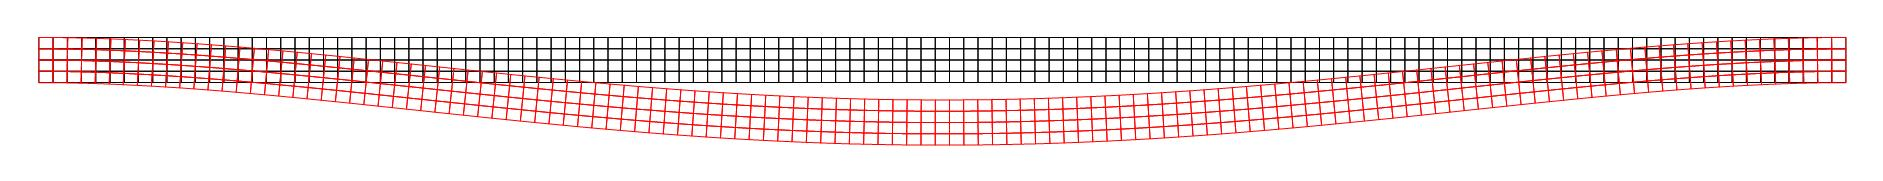
\includegraphics[width=1\textwidth]{1}
			\captionof*{figure}{\textbf{Obrázek 1.} Mathematica (pevné konce)}
		\end{minipage}
		\begin{minipage}[b]{0.5\textwidth}
			\centering
			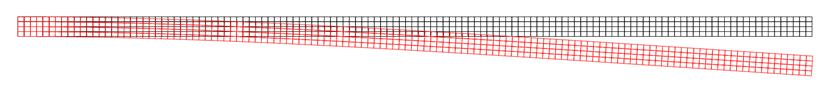
\includegraphics[width=1\textwidth]{2}
			\captionof*{figure}{\textbf{Obrázek 2.} Mathematica (pevný konec)}
		\end{minipage}
		\hfill
	\end{minipage}
	\begin{minipage}{\textwidth}
		\begin{minipage}[b]{0.5\textwidth}
			\centering
			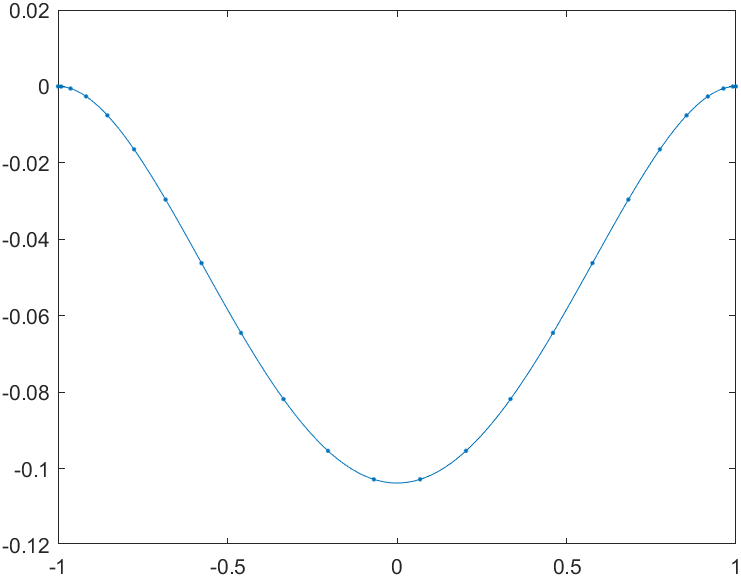
\includegraphics[width=0.7\textwidth]{untitled1}
			\captionof*{figure}{\textbf{Obrázek 3.} Matlab (pevné konce)}
		\end{minipage}
		\begin{minipage}[b]{0.5\textwidth}
			\centering
			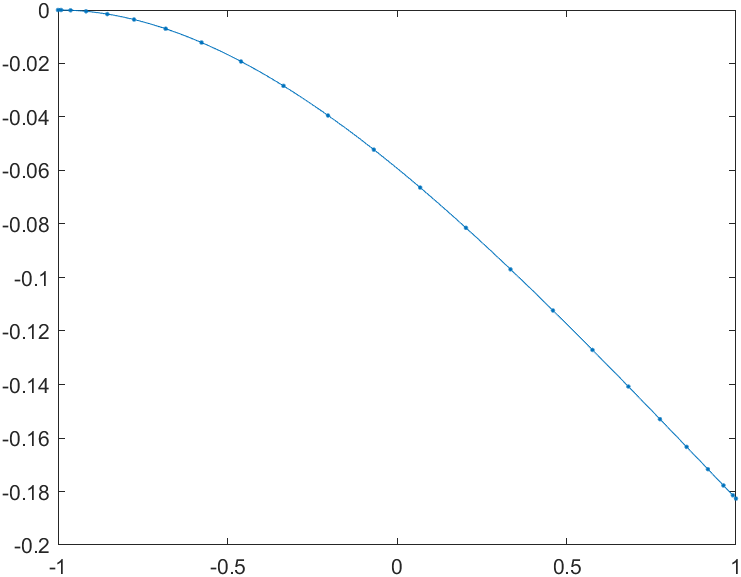
\includegraphics[width=0.7\textwidth]{untitled2}
			\captionof*{figure}{\textbf{Obrázek 4.} Matlab (pevný konec)}
		\end{minipage}
		\hfill
	\end{minipage}
\end{frame}
\begin{frame}
	\frametitle{Vibrace destičky}
	
	{\tiny'Najprimitívnejší model pre vychýlenie dosiek je daný rovnicou'
	\begin{equation}
		\label{eq:2}
		\frac{\partial ^2{u}}{\partial {t^{2}}}-K^{2}\Delta{u}=0,
	\end{equation}
	"kde $u$ je vychýlenie dané ako zobrazenie $u:(t,\vec{x}) \in \mathbb{R} \times \mathbb{R}^{2} \mapsto \mathbb{R}$"
	"Pre stojaté vlnenie má riešenie \eqref{eq:2} tvar:"
	\begin{equation}
		\label{eq:3}
		-\Delta{\widehat{u}}=\frac{\omega^{2}}{K^{2}}\widehat{u}
	\end{equation}
	"Ak označíme $L=_{def}-\Delta$ a $\lambda=_{def}\frac{\omega^{2}}{K^{2}}$ z \ref{eq:3} dostaneme:"
	\begin{equation}
		\label{eq:4}
		-L{\widehat{u}}=\lambda\widehat{u}
	\end{equation}
	"Z čoho dostaneme po dosadení vhodných okrajových podmienok úlohu pre nájdenie vlastných vektorov lineárneho operátora."
		"Chceme nájsť vlastné vektory a vlastné čísla Laplaceovho operátora v $\Omega \subset \mathbb{R}^{2}$ s nulovou Dirichletovou podmienkou. Chceme teda riešiť:"
	
	\begin{subeqations}
		\label{eq:5}
		\begin{equation}
			\label{eq:6}
			-\Delta{\widehat{u}}=\lambda\widehat{u}
		\end{equation}
		
		\begin{equation}
			\label{eq:7}
			\widehat{u}|_{\partial{\Omega}}=0
		\end{equation}
		
	\end{subeqations}
	Hodnoty \widehat{u} v interpolačných $[x_{i},y_{k}]$ bodoch označíme ako $\widehat{u}_{i,k}$, dostávame:
	
	\begin{equation}
		\label{eq:8}
		\widehat{u}_{i,k}=_{def}(\widehat{u}_{x})_{i,k}=_{def}\widehat{u}(x_i,y_k).
	\end{equation}
	
	Aproximácie parciálnych derivácií podľa x a y budú označené ako $(\widehat{u}_{x})_{i,k}$ a $(\widehat{u}_{y})_{i,k}$. Teda
	\begin{subequations}
		\label{eq:9}
		\begin{equation}
			\label{eq:10}
			(\widehat{u}_{x})_{i,k}=_{def}\frac{\partial \widehat{u} }{\partial x}(x,y)\mid_{x=x_i,y=y_k}
		\end{equation}
		\begin{equation}
			\label{eq:11}
			(\widehat{u}_{y})_{i,k}=_{def}\frac{\partial \widehat{u} }{\partial y}(x,y)\mid_{x=x_i,y=y_k}.
		\end{equation}
	\end{subequations}
	}
\end{frame}


\section*{Vibrace destičky}
\label{sec:desticka}

\begin{frame}
	\frametitle{Vlastní čísla}
	{\tiny V následujích výpočtech jsme vždy uvažovali obdélník $2 \times 3$, s čímž nám vyšla následující vlastní čísla:}\\
		\begin{minipage}[b]{1\textwidth}
			\centering
			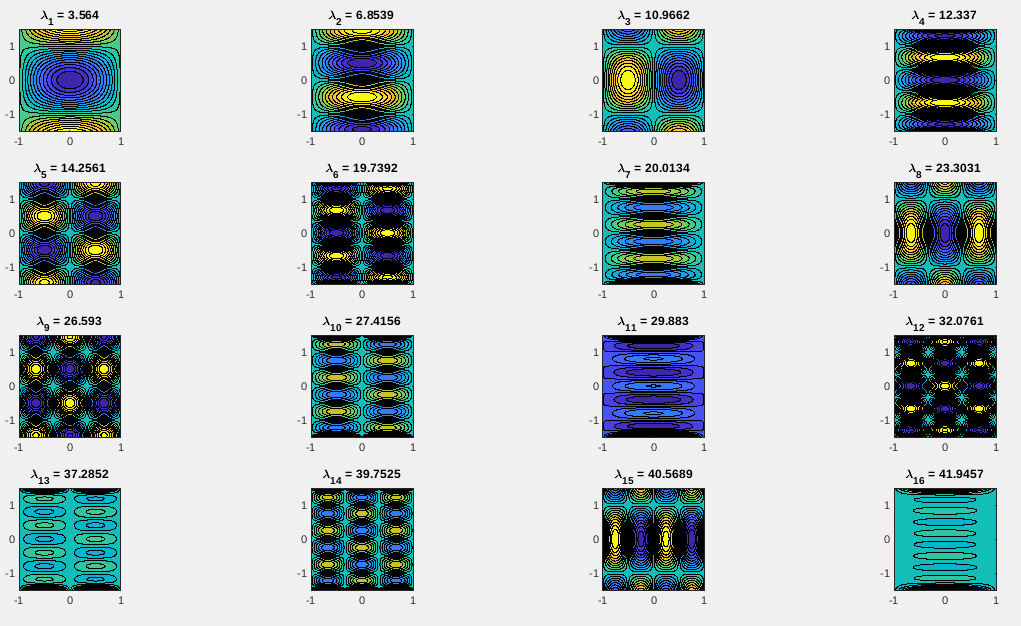
\includegraphics[width=0.9\textwidth]{barevne.png}
			\captionof*{figure}{\textbf{Obrázek 5.} Vlastní čísla pro obdelník}
		\end{minipage}
\end{frame}
\begin{frame}
	\frametitle{Matlab vs Mathematica}
	Pro ukázku tady ještě máme několik vlastních čísel toho samého v $Mathematice$.
	\begin{figure}[h!]
		\centering
		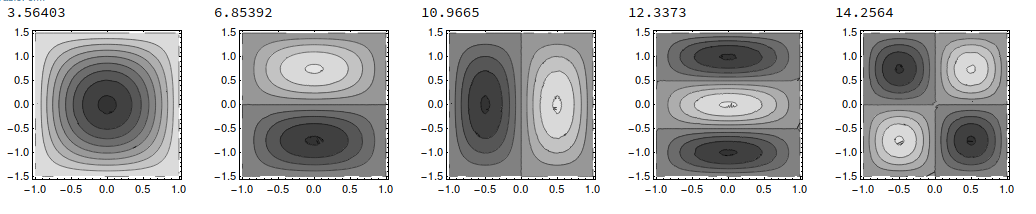
\includegraphics[width = 1\textwidth]{mathematica1.png}
		\caption*{\textbf{Obrázek 6.} Vlastní čísla v Mathematice}
	\end{figure}
\end{frame}


\end{document}
